% Section content template for individual Educative lessons
% This file contains the actual content for a specific section
% Generated from Educative API section content

% Section: Introduction to the Design Patterns
% Section ID: 5742887740637184
% Section Slug: introduction-to-the-design-patterns
% Generated: 2025-12-11T06:15:42.414327

\subsection{What are design patterns?}\label{what-are-design-patterns}
\\
Designing efficient and reusable code is something that all developers strive for. When working on large applications, code structure becomes an integral element where we need to prevent repeating code for similar tasks. However, trying to build upon and adding features to an existing system is quite a challenging task, since a developer needs to know the complete particulars. These include the relationships that each entity possesses or the sort of hierarchy that exists between different entities. Also , developers need to update their code in such a way as to make it easily adaptable to change in the future. In such scenarios, it'll be helpful to have a structure that could be used to solve various common issues. This is where the design patterns come into play.
\\
\textbf{Design patterns} are solutions to frequently occurring real-life problems in software design. They can also be considered customizable templates that can meet the requirements of a particular design problem. Let's take the example of an ice-cream factory that serves as the base of operations to produce various types of ice creams according to the defined requirements. This is similar to how a design pattern can be used as a template in different circumstances.

\begin{figure}[htbp]
 \centering
 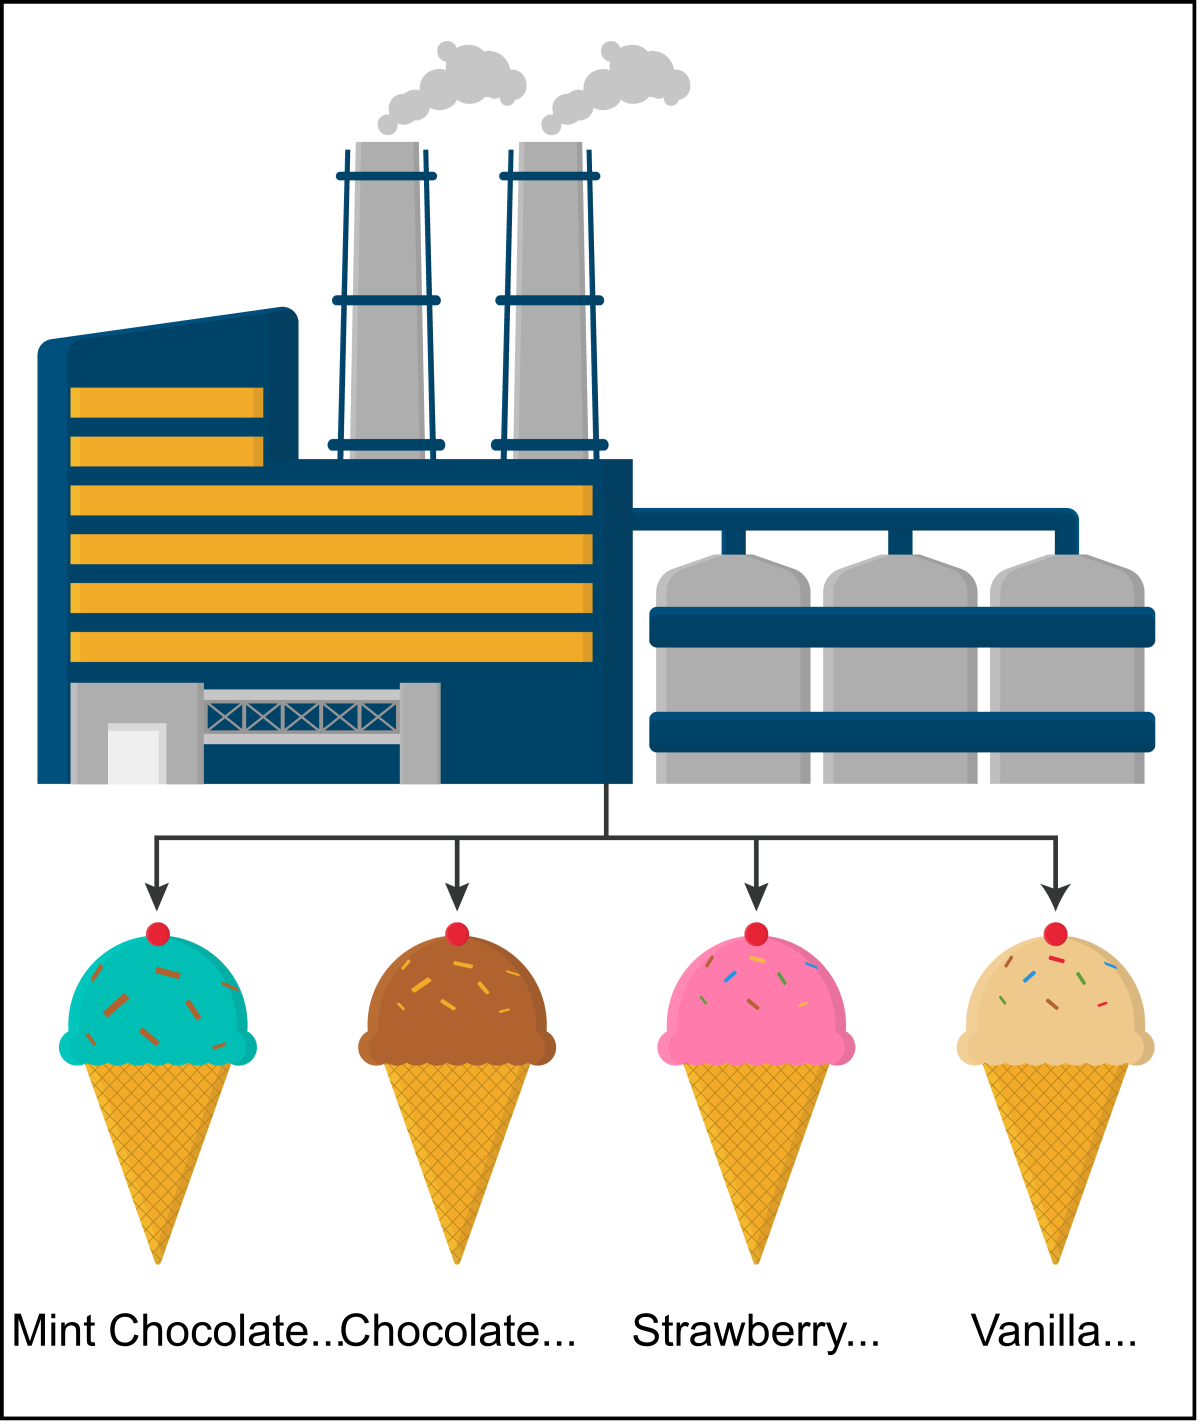
\includegraphics[width=0.25\textwidth]{Images/chapter_5/section_5742887740637184/4937143928750080.png}
 \caption{A real-life example of the design patterns}
\end{figure}

\subsection{Structure of design patterns}\label{structure-of-design-patterns}

\begin{itemize}
\item
\textbf{Pattern name:} This is an identification step that describes a design problem.
\item
\textbf{Intent:} This step describes the use case of the particular design pattern.
\item
\textbf{Motivation:} This step illustrates the problem and talks about the inner components in the pattern to solve the problem.
\item
\textbf{Structure:} This step visualizes the structure using a graphical representation of the classes in the pattern.
\item
\textbf{Consequences:} This step describes the trade-offs of a particular pattern.
\item
\textbf{Implementation:} This step illustrates an example of code in any popular programming language.
\end{itemize}

\subsection{Advantages of design patterns}\label{advantages-of-design-patterns}
\\
The following are some of the advantages of using design patterns:

\begin{itemize}
\item
They provide correct and efficient solutions since they have been derived and optimized by various experienced programmers over time.
\item
They are generic templates that can be modified and used for solving different problems.
\item
They can provide a clean and elegant solution to a large problem by avoiding repetition in the code.
\item
They provide a template on which the developers can build upon. This allows developers to spend less time on code structure and more on the overall quality of the solution.
\end{itemize}

\subsection{Consequences of unfamiliarity with the design patterns}\label{consequences-of-unfamiliarity-with-the-design-patterns}
\\
While there are many advantages of using design patterns, it is important to fully understand the depths of design patterns, since unfamiliarity might cause the following issues:

\begin{itemize}
\item
Design patterns can complicate the architecture of the application if they are managed poorly.
\item
Developers who are not familiar with them might end up getting confused as to why certain patterns are being used.
\end{itemize}
\\
Now that we've gotten a flavor of what design patterns are, let's explore some of their different types in the next lesson.

% End of section content